\documentclass{article}

\usepackage{graphicx} % Required for inserting images
\usepackage{amsmath}
\usepackage{amssymb}
\usepackage{amsthm}
\usepackage{amsfonts}
\usepackage{tcolorbox}
\usepackage{tikz}
\usetikzlibrary{calc, intersections, through, backgrounds}
\usepackage{tkz-euclide}
\usetikzlibrary{graphs}
\usepackage{multicol}
\usepackage{pgfplots}
\pgfplotsset{compat=1.18} % Use the latest compatibility for pgfplots
\usepackage{tabularx}
\usepackage{import}
\usepackage{lipsum}
\usepackage{fancyhdr} 
\usepackage{wrapfig}
\usepackage{mwe}
\usepackage[export]{adjustbox}
\usepackage{subcaption}
\usepackage{caption}
\usepackage{gensymb}

\newtheorem{theorem}{Theorem}
\newtheorem{exercise}{Excercise}
\newtheorem{question}{Question}
\newtheorem{lemma}{Lemma}
\newtheorem{problem}{Problem}
\newtheorem{definition}{Def}

\renewcommand\qedsymbol{$\blacksquare$}

\newcommand{\tarc}{\frown}
\newcommand{\arc}[1]{\stackrel{\tarc}{#1}}

\author{Daniel Mineev}
\title{Sawayama's Lemma and Thebault's circles}
\date{}

\begin{document}

\maketitle

This paper compiles a collection of geometric proofs and related constructions that center around Sawayama's Lemma and Thébault's theorem. The document begins with the presentation and proof of the Shooting Lemma, which establishes a relationship between a chord in a circle, a tangent circle, and the midpoint of the larger arc. Using this foundational lemma, the proofs of Sawayama's Lemma and Verrier's Lemma follow, demonstrating the collinearity of specific points associated with inscribed triangles and tangent circles. The final section extends these results to prove Thébault's theorem, generalizing the principles of Sawayama's and Verrier's Lemmas to a broader context involving two tangent circles.

\section{The Shooting Lemma}

\begin{theorem}
	Consider the chord \(BC\) in the circle \(\Omega\). Let the circle \(\omega\) touch \(BC\) at a point \(D\) and the circle \(\Omega\) at a point \(E\). Prove that the line \(DE\) passes through \(M\), the middle of the larger arc \(\arc{BC}\).
\end{theorem}

\begin{center}
    \centering
    \begin{tikzpicture}[scale=0.6]
        \tkzDefPoints{0/0/O,3/1/B,-3/1/C}
        \tkzDrawCircle(O,B)
        \tkzDrawPoints(B,C)
        \tkzLabelPoints[above right](B)
        \tkzLabelPoints[above left](C)
        
        \tkzDrawLine(B,C)
        
        \tkzDefMidArc(O,C,B) \tkzGetPoint{M}
        
        \tkzDrawPoint(M)
        \tkzLabelPoints[below right](M)
        
        \tkzDefPointOnCircle[through = center O angle 60 point B] \tkzGetPoint{E}
        
        \tkzDrawPoint(E)
        \tkzLabelPoints[above right](E)
        
        \tkzInterLL(C,B)(E,M) \tkzGetPoint{D}
        \tkzDrawPoint(D) \tkzLabelPoints[below right](D)
        
        % Calculate ED and EM
        \tkzCalcLength(E,D) \tkzGetLength{ED}
        \tkzCalcLength(E,M) \tkzGetLength{EM}
        \pgfmathsetmacro{\ratioo}{\ED/\EM} % Correct the syntax for defining the ratio

        % Define the homothety with the calculated ratio
        \tkzDefPointBy[homothety=center E ratio \ratioo](C) \tkzGetPoint{CC'}
        \tkzDefCircle[circum](E,D,CC') \tkzGetPoint{O}
	\tkzDrawCircle(O,E)
	
	\tkzDrawLine[dashed, blue](E,M)
    \end{tikzpicture}
\end{center}

\begin{proof}
The proof is quite trivial, simply consider the homothety centered at \(E\), which transforms \(\omega\) into \(\Omega\). Then, \(B\) is mapped to \(B'\) and \(C\) to \(C'\), where \(B'\) and \(C'\) are the intersections of \(CE\) and \(BE\) with the tangent from \(M\) to \(\Omega\) respectevely.

\begin{center}
    \centering
    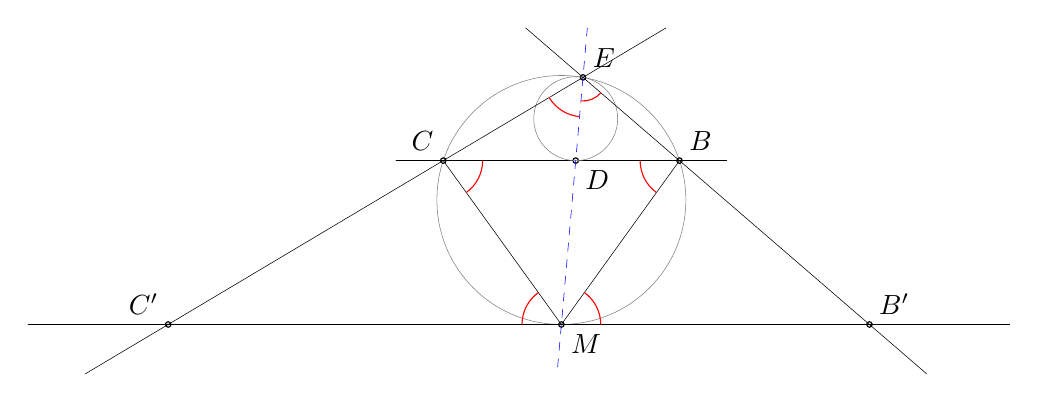
\begin{tikzpicture}[scale=0.5]
        \tkzDefPoints{0/0/O,3/1/B,-3/1/C}
        \tkzDrawCircle(O,B)
        \tkzDrawPoints(B,C)
        \tkzLabelPoints[above right](B)
        \tkzLabelPoints[above left](C)
        
        \tkzDrawLine(B,C)
        
        \tkzDefMidArc(O,C,B) \tkzGetPoint{M}
        
        \tkzDrawPoint(M)
        \tkzLabelPoints[below right](M)
        
        \tkzDefPointOnCircle[through = center O angle 80 point B] \tkzGetPoint{E}
        
        \tkzDrawPoint(E)
        \tkzLabelPoints[above right](E)
        
        \tkzInterLL(C,B)(E,M) \tkzGetPoint{D}
        \tkzDrawPoint(D) \tkzLabelPoints[below right](D)
        
        % Calculate ED and EM
        \tkzCalcLength(E,D) \tkzGetLength{ED}
        \tkzCalcLength(E,M) \tkzGetLength{EM}
        \pgfmathsetmacro{\ratioo}{\ED/\EM} % Correct the syntax for defining the ratio

        % Define the homothety with the calculated ratio
        \tkzDefPointBy[homothety=center E ratio \ratioo](C) \tkzGetPoint{CC'}
        \tkzDefCircle[circum](E,D,CC') \tkzGetPoint{O}
	\tkzDrawCircle(O,E)
	
	\tkzDrawLine[dashed, blue](E,M)
	
	% Definition of B' and C'
         \pgfmathsetmacro{\ratio}{\EM/\ED} 
        
	\tkzDefPointBy[homothety=center E ratio \ratio](C) \tkzGetPoint{C'}
	\tkzDrawPoint(C') \tkzLabelPoints[above left](C')
	
	\tkzDefPointBy[homothety=center E ratio \ratio](B) \tkzGetPoint{B'}
	\tkzDrawPoint(B') \tkzLabelPoints[above right](B')

	\tkzDrawLines(E,C' E,B')
	\tkzDrawLine(C',B')
	
	\tkzDrawSegments(C,M B,M)
	
	\tkzMarkAngle[arc=l, color = red](C,M,C')
	\tkzMarkAngle[arc=l, color = red](M,C,B)
	\tkzMarkAngle[arc=l, color = red](C,B,M)
	\tkzMarkAngle[arc=l, color = red](B',M,B)
	\tkzMarkAngle[arc=l, color = red](C,E,M)
	\tkzMarkAngle[arc=l, color = red, size=0.6](M,E,B)
    \end{tikzpicture}
 \end{center}
 
 Then, \(\angle{BCM} = \angle{CMC'}\) due to \(CB \parallel C'B'\), and \(\angle{CBM} = \angle{CMC'}\) because \(C'B'\) touches \(\Omega\) and finally \(\angle{CBM} = \angle{BMB'}\). Thus, \(\angle{CMC'} = \angle{BMB'}\), however due to \(\Omega\) touching \(C'B'\) we know that \(\angle{CEM} = \angle{CMC'}\) and \(\angle{BEM} = \angle{BMB'}\), consequently \(\angle{CEM} = \angle{MEB}\). In other words \(ME\) is the bisector of \(\angle{CEB}\) which means that \(M\) is the middle of the larger arc \(\arc{BC}\).
 
 \end{proof}
    
In fact, due to \(\angle{BEM} = \angle{DBM}\) we conclude that \((EDB)\) touches \(BM\), consequently,

\begin{equation}
    pow_{(EDB)} M = MD \cdot ME = MB^2
\end{equation}
    
And due to \(M\) being the middle of \(\arc{BC}\) it must be that \(CM = MB\), thus, \(MB^2 = MC \cdot MB\). Combining these results we get a nice formula,
\begin{equation}
    MC \cdot MB = MD \cdot ME
\end{equation}

The figure can also show a lot of interesting and fundemental properties if one performs an inversion centered at the point \(M\) with a radius of \(MB = MC\). Then through this process \(\Omega \leftrightarrow BC\) and because \(\omega\) must continue to touch \(inv(BC)\) and \(inv(\Omega)\) (in other words \(\Omega\) and \(BC\)) and it must be in the same angle from \(M\), it must be the case that \(\omega \rightarrow \omega\) under the inversion. Consequently, it must mean that \(D \leftrightarrow E\) and thus \(M, D\) and \(E\) are colinear. Another consequence of such argument is that the length of the tangents from \(M\) to \(\omega\) are equal to \(MB = MC\).

Now let us consider the following, a bit stronger statement,

\begin{theorem}
Let \(A\) be an arbitrary point on the arc \(\arc{CEB}\) and let \(I\) be an arbitrary point on \(AM\). Let \(L\) be the intersection of \(ID\) and \(\omega\), prove that \(AILE\) is cyclic.
\end{theorem}

\begin{center}
    \centering
    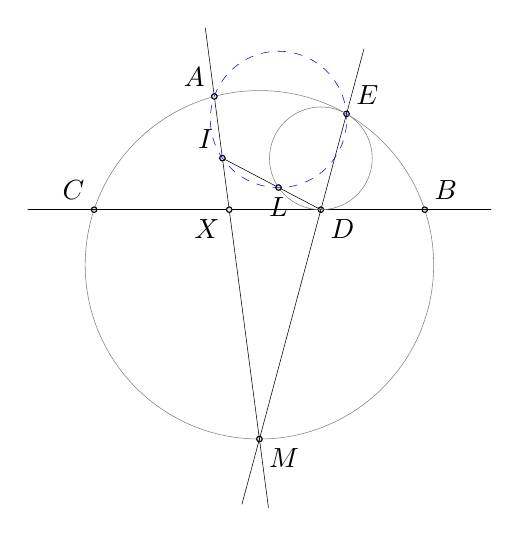
\begin{tikzpicture}[scale=0.7]
        \tkzDefPoints{0/0/O,3/1/B,-3/1/C}
        \tkzDrawCircle(O,B)
        \tkzDrawPoints(B,C)
        \tkzLabelPoints[above right](B)
        \tkzLabelPoints[above left](C)
        
        \tkzDrawLine(B,C)
        
        \tkzDefMidArc(O,C,B) \tkzGetPoint{M}
        
        \tkzDrawPoint(M)
        \tkzLabelPoints[below right](M)
        
        \tkzDefPointOnCircle[through = center O angle 60 point B] \tkzGetPoint{E}
        \tkzDefPointOnCircle[through = center O angle 105 point B] \tkzGetPoint{A}
        
        \tkzDrawLine(A,M)
        
        \tkzDrawPoint(E) \tkzDrawPoint(A)
        \tkzLabelPoints[above right](E)
        \tkzLabelPoints[above left](A)
        
        \tkzInterLL(C,B)(E,M) \tkzGetPoint{D}
        \tkzInterLL(A,M)(C,B) \tkzGetPoint{X}
        \tkzDrawPoints(D,X) \tkzLabelPoints[below right](D) \tkzLabelPoints[below left](X)
        
        % Calculate ED and EM
        \tkzCalcLength(E,D) \tkzGetLength{ED}
        \tkzCalcLength(E,M) \tkzGetLength{EM}
        \pgfmathsetmacro{\ratioo}{\ED/\EM} % Correct the syntax for defining the ratio

        % Define the homothety with the calculated ratio
        \tkzDefPointBy[homothety=center E ratio \ratioo](C) \tkzGetPoint{CC'}
        \tkzDefCircle[circum](E,D,CC') \tkzGetPoint{O}
	\tkzDrawCircle(O,E)
	
	\tkzDrawLine(E,M)
        
        \tkzDefPointWith[linear,K=0.18](A,M) \tkzGetPoint{I}
        \tkzDrawSegment(I,D)
        
        \tkzInterLC(I,D)(O,E) \tkzGetPoints{L}{X}
        
        \tkzDrawPoints(L) \tkzLabelPoints(L)
        
        \tkzDrawPoint(I) \tkzLabelPoints[above left](I)
        
        \tkzDefCircle[circum](A,I,L) \tkzGetPoint{OO}
	\tkzDrawCircle[dashed, blue](OO,A)
    \end{tikzpicture}
\end{center}

\begin{proof}

This is also quite a trivial statement, noticing from the previous statement that \(CM^2 = MX \cdot AM\) and \(CM^2 = MD \cdot ME\) we can conclude that \(MX \cdot MA = MD \cdot ME\) which by the power of the point \(M\) concludes that \(AXDE\) is cyclic. Now, all that is left to notice is that, \(\angle{ELD} = \angle{EDB}\) due to \(DB\) touching \(\omega\) and \(\angle{EDB} = \angle{EAX}\) due to \(AXED\) being cyclic, thus \(\angle{IAE} = \angle{ELD}\) and \(AILE\) is cyclic.

\end{proof}

It is a bit interesting to see the behaviour of \((AILE)\) as one moves \(I\) along \(AM\). When \(I = X\) we get an already proven statement that \(AXDE\) is cyclic and when \(I = A\) we see that \((AILE)\) touches \(ED\). However, there is a more important position of \(I\) which has the following property.

\begin{lemma}
If \(MI = BM = CM\), then \(AL\) tangent to \(\omega\).
\end{lemma}
\begin{proof}
This again is no less trivial than the last statement, simply notice that \(MD \cdot ME = MC^2 = MI^2\), thus \((IDE)\) touches \(AM\). Consequently,

\begin{equation}
\angle{IDE} = \angle{AIE} = \angle{ALE}
\end{equation}

due to \(AILE\) being cyclic. Which implies that \(AL\) touches \(\omega\).
\end{proof}

\section{Sawayama's and Verrier's Lemma's}

\begin{theorem} \textbf{(Sawayama's lemma)}
Let \(\triangle ABC\) be inscribed into \(\Omega\) and let \(X\) be an arbitrary point \(AB\). Consider \(\omega\) which is tangent to the segment \(XC\), the segment \(XB\) and \(\Omega\). Let \(L\) and \(K\) be the tangency points of \(\omega\) with \(XC\) and \(XB\) respectively. Prove that \(L\), \(K\) and \(I\) (the incenter of \(\triangle ABC\)) are colinear.
\end{theorem}

\begin{center}
    \centering
    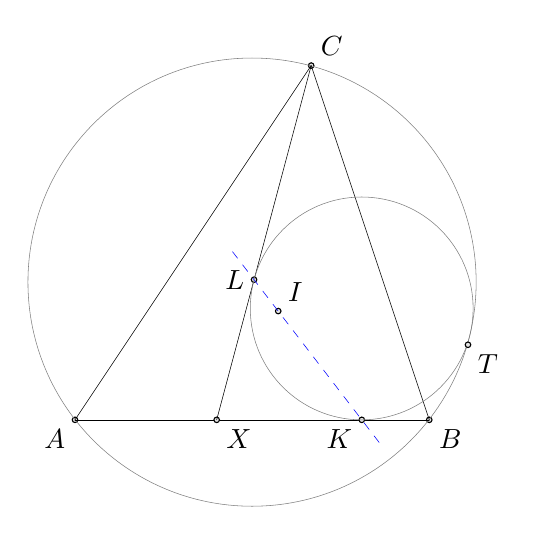
\begin{tikzpicture}[scale=1.5]
        \tkzDefPoints{0/0/A,3/0/B,2/3/C}
        \tkzDrawPoints(A,B,C) \tkzLabelPoints[below left](A) \tkzLabelPoints[below right](B) \tkzLabelPoints[above right](C)
        
        \tkzDefCircle[circum](A,B,C) \tkzGetPoint{O}
	\tkzDrawCircle(O,A)
	
	\tkzDrawSegments(A,C B,C A,B)
	\tkzDefPointWith[linear,K=0.4](A,B) \tkzGetPoint{X}
	\tkzDrawPoint(X) \tkzLabelPoints[below right](X)
	\tkzDrawSegment(C,X)
	
	\tkzDefTriangleCenter[in](A,B,C) \tkzGetPoint{I}
	\tkzDrawPoints(I) \tkzLabelPoints[above right](I)
	
	\tkzDefLine[bisector](C,X,B) \tkzGetPoint{x}
	
	\tkzDefLine[perpendicular=through I](X,x) \tkzGetPoint{c}
	
	\tkzInterLL(A,B)(I,c) \tkzGetPoint{K}
	\tkzInterLL(X,C)(I,c) \tkzGetPoint{L}
	
	\tkzDrawPoints(K,L)
	\tkzLabelPoints[left](L)
	\tkzLabelPoints[below left](K)
	
	\tkzDefLine[perpendicular=through L](X,C) \tkzGetPoint{cc}
	\tkzDefLine[perpendicular=through K](A,B) \tkzGetPoint{ccc}
	
	\tkzInterLL(L,cc)(K,ccc) \tkzGetPoint{O'}
	\tkzDrawCircle(O',K)

	\tkzInterCC[common=B](O,B)(O',K) \tkzGetFirstPoint{T}
	
	\tkzDrawPoint(T) \tkzLabelPoints[below right](T)
	
	\tkzDrawLine[dashed, blue](L,K)
    \end{tikzpicture}
\end{center}

\begin{proof}
Now it is time to utilize all the lemmas proven in the previous section. The first step is to extend \(CI\) till the intersection with \(\Omega\), let that intersection point be \(P\). Then, due to the Trillium theorem it is clear that \(PI = AP = PB\). This allows one to apply the last lemma to this configuration. Here \(C\) is serves as the arbitrary point from the last lemma and due to \(IP = AP = PB\) it must be that the intersection of \(IK\) with \(\omega\), let that point be \(L'\), must be the tangency point from \(C\) to \(\omega\). 

\begin{center}
    \centering
    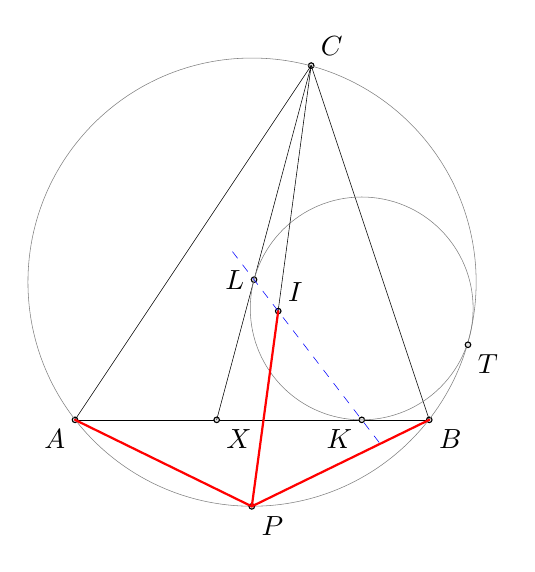
\begin{tikzpicture}[scale=1.5]
        \tkzDefPoints{0/0/A,3/0/B,2/3/C}
        \tkzDrawPoints(A,B,C) \tkzLabelPoints[below left](A) \tkzLabelPoints[below right](B) \tkzLabelPoints[above right](C)
        
        \tkzDefCircle[circum](A,B,C) \tkzGetPoint{O}
	\tkzDrawCircle(O,A)
	
	\tkzDrawSegments(A,C B,C A,B)
	\tkzDefPointWith[linear,K=0.4](A,B) \tkzGetPoint{X}
	\tkzDrawPoint(X) \tkzLabelPoints[below right](X)
	\tkzDrawSegment(C,X)
	
	\tkzDefTriangleCenter[in](A,B,C) \tkzGetPoint{I}
	\tkzDrawPoints(I) \tkzLabelPoints[above right](I)
	
	\tkzDefLine[bisector](C,X,B) \tkzGetPoint{x}
	
	\tkzDefLine[perpendicular=through I](X,x) \tkzGetPoint{c}
	
	\tkzInterLL(A,B)(I,c) \tkzGetPoint{K}
	\tkzInterLL(X,C)(I,c) \tkzGetPoint{L}
	
	\tkzDrawPoints(K,L)
	\tkzLabelPoints[left](L)
	\tkzLabelPoints[below left](K)
	
	\tkzDefLine[perpendicular=through L](X,C) \tkzGetPoint{cc}
	\tkzDefLine[perpendicular=through K](A,B) \tkzGetPoint{ccc}
	
	\tkzInterLL(L,cc)(K,ccc) \tkzGetPoint{O'}
	\tkzDrawCircle(O',K)

	\tkzInterCC[common=B](O,B)(O',K) \tkzGetFirstPoint{T}
	
	\tkzDrawPoint(T) \tkzLabelPoints[below right](T)
	
	\tkzDrawLine[dashed, blue](L,K)
	
	\tkzInterLC(C,I)(O,A) \tkzGetPoints{P}{Q}
	\tkzDrawPoint(P) \tkzLabelPoints[below right](P) \tkzDrawSegment(C,P)
	
	\tkzDrawSegments[red, thick](A,P P,B P,I)
    \end{tikzpicture}
\end{center}

However, that tangency point is \(L\) by definition, thus \(L' = L\) and consequently \(L\), \(I\) and \(K\) are colinear.

\end{proof}

Now consider what happens when one moves \(X\) along \(AB\), specifically let \(X = A\). Then, Sawayama's lemma will transform itself into Verrier's lemma.

\begin{theorem} \textbf{(Verrier's lemma)}
Let \(\triangle ABC\) be inscribed into \(\Omega\) and let \(\omega\) be a circle which is tangent to the segments \(BC\), \(AB\) and \(\Omega\) at points \(L\), \(K\) and \(T\) respectively. Then, \(L\), \(K\) and \(I\) (incenter of \(\triangle ABC\)) are colinear. 
\end{theorem}

\begin{center}
    \centering
    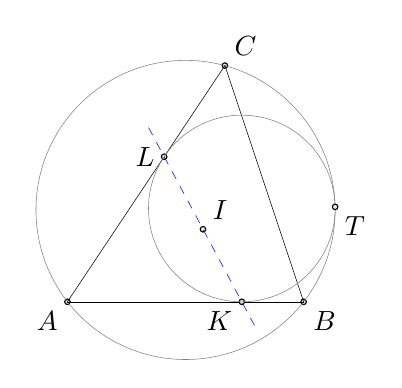
\begin{tikzpicture}[scale=1]
        \tkzDefPoints{0/0/A,3/0/B,2/3/C}
        \tkzDrawPoints(A,B,C) \tkzLabelPoints[below left](A) \tkzLabelPoints[below right](B) \tkzLabelPoints[above right](C)
        
        \tkzDefCircle[circum](A,B,C) \tkzGetPoint{O}
	\tkzDrawCircle(O,A)
	
	\tkzDrawSegments(A,C B,C A,B)
	\tkzDefPointWith[linear,K=0](A,B) \tkzGetPoint{X}
	
	\tkzDefTriangleCenter[in](A,B,C) \tkzGetPoint{I}
	\tkzDrawPoints(I) \tkzLabelPoints[above right](I)
	
	\tkzDefLine[bisector](C,X,B) \tkzGetPoint{x}
	
	\tkzDefLine[perpendicular=through I](X,x) \tkzGetPoint{c}
	
	\tkzInterLL(A,B)(I,c) \tkzGetPoint{K}
	\tkzInterLL(X,C)(I,c) \tkzGetPoint{L}
	
	\tkzDrawPoints(K,L)
	\tkzLabelPoints[left](L)
	\tkzLabelPoints[below left](K)
	
	\tkzDefLine[perpendicular=through L](X,C) \tkzGetPoint{cc}
	\tkzDefLine[perpendicular=through K](A,B) \tkzGetPoint{ccc}
	
	\tkzInterLL(L,cc)(K,ccc) \tkzGetPoint{O'}
	\tkzDrawCircle(O',K)

	\tkzInterCC[common=B](O,B)(O',K) \tkzGetFirstPoint{T}
	
	\tkzDrawPoint(T) \tkzLabelPoints[below right](T)
	
	\tkzDrawLine[dashed, blue](L,K)
    \end{tikzpicture}
\end{center}

This statement has other proofs which do not involve Sawayama's lemma, one of the most notable ones is the following which showcases the mechanism at play.

\begin{proof}
Let us intersect \(TL\) and \(TK\) with \(\Omega\) in points \(M_1\) and \(M_2\), by the shooting lemma it must be that \(M_1\) and \(M_2\) are the middle's of arcs \(\arc{AB}\) and \(\arc{AC}\). Consequently they must lie on the lines \(BI\) and \(CI\).

\begin{center}
    \centering
    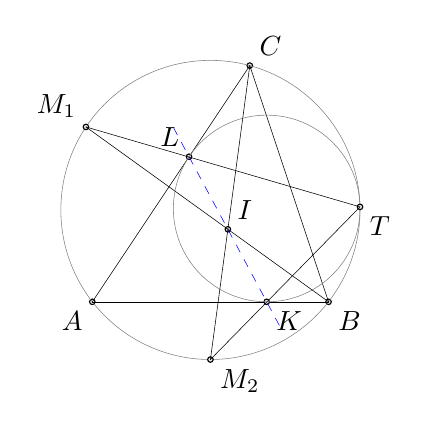
\begin{tikzpicture}[scale=1]
        \tkzDefPoints{0/0/A,3/0/B,2/3/C}
        \tkzDrawPoints(A,B,C) \tkzLabelPoints[below left](A) \tkzLabelPoints[below right](B) \tkzLabelPoints[above right](C)
        
        \tkzDefCircle[circum](A,B,C) \tkzGetPoint{O}
	\tkzDrawCircle(O,A)
	
	\tkzDrawSegments(A,C B,C A,B)
	\tkzDefPointWith[linear,K=0](A,B) \tkzGetPoint{X}
	
	\tkzDefTriangleCenter[in](A,B,C) \tkzGetPoint{I}
	\tkzDrawPoints(I) \tkzLabelPoints[above right](I)
	
	\tkzDefLine[bisector](C,X,B) \tkzGetPoint{x}
	
	\tkzDefLine[perpendicular=through I](X,x) \tkzGetPoint{c}
	
	\tkzInterLL(A,B)(I,c) \tkzGetPoint{K}
	\tkzInterLL(X,C)(I,c) \tkzGetPoint{L}
	
	\tkzDrawPoints(K,L)
	\tkzLabelPoints[above left](L)
	\tkzLabelPoints[below right](K)
	
	\tkzDefLine[perpendicular=through L](X,C) \tkzGetPoint{cc}
	\tkzDefLine[perpendicular=through K](A,B) \tkzGetPoint{ccc}
	
	\tkzInterLL(L,cc)(K,ccc) \tkzGetPoint{O'}
	\tkzDrawCircle(O',K)

	\tkzInterCC[common=B](O,B)(O',K) \tkzGetFirstPoint{T}
	
	\tkzDrawPoint(T) \tkzLabelPoints[below right](T)
	
	\tkzDrawLine[dashed, blue](L,K)
	
	\tkzInterLC(B,I)(O,A) \tkzGetPoints{M_1}{M_1'}
	\tkzInterLC(C,I)(O,A) \tkzGetPoints{M_2}{M_2'}
	
	\tkzDrawPoints(M_1, M_2) \tkzLabelPoints[above left](M_1) \tkzLabelPoints[below right](M_2)
	
	\tkzDrawSegments(T,M_1 B,M_1 C,M_2 T,M_2)
    \end{tikzpicture}
\end{center}

All that is left is to apply Pascal's theorem for \(M_1 A M_2 B T C\) and conclude that \(L\), \(I\) and \(K\) are colinear.

\end{proof}

A beautiful lemma about the \(M_1 M_2\) is the following,

\begin{lemma}
The radical axis of \((A,0)\) (the circle centered at \(A\) with a radius of zero) and \(\omega\) is \(M_1 M_2\).
\end{lemma}

\begin{proof}
Notice that due to the shooting lemma and its consequences, it must be that \(M_1A^2 = M_1 L \cdot M_1 T\) and \(M_2 A^2 = M_2 K \cdot M_2 T\). This, means that,
\begin{equation}
pow_{(A,0)} M_1 = M_1^2 = M_1 L \cdot M_1 T = pow_{\omega} M_1 \\
\end{equation}
\begin{equation}
pow_{(A,0)} M_2 = M_2^2 = M_2 K \cdot M_2 T = pow_{\omega} M_2
\end{equation}
Thus, it must be that \(M_1\) and \(M_2\) lie on the radical axis of \((A,0)\) and \(\omega\), in other words \(M_1 M_2\) is the radical axis of \((A,0)\) and \(\omega\).

\end{proof}

\section{Thebault's theorem}

\begin{theorem} \textbf{(Thebault's theorem)}
If \(\triangle ABC\) is inscribed into \(\Omega\), let \(\omega_1\) be the circle tangent to the segments \(XB\) and \(XC\) and \(\Omega\) and let the circle \(\omega_2\) be the circle tangent to the segments \(XC\), \(AX\) and \(\Omega\). Let \(O_1\) and \(O_2\) be the centers of \(\omega_1\) and \(\omega_2\). Then, \(O_1\), \(O_2\) and \(I\) (the incenter of \(\triangle ABC\)) are colinear.
\end{theorem}


\begin{center}
    \centering
    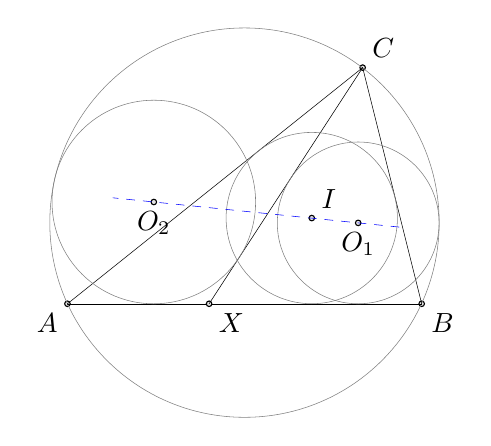
\begin{tikzpicture}[scale=1.5]
        \tkzDefPoints{0/0/A,3/0/B,2.5/2/C}
        \tkzDrawPoints(A,B,C) \tkzLabelPoints[below left](A) \tkzLabelPoints[below right](B) \tkzLabelPoints[above right](C)
        
        \tkzDefCircle[circum](A,B,C) \tkzGetPoint{O}
	\tkzDrawCircle(O,A)
	
	\tkzDrawSegments(A,C B,C A,B)
	\tkzDefPointWith[linear,K=0.4](A,B) \tkzGetPoint{X}
	\tkzDrawPoint(X) \tkzLabelPoints[below right](X)
	\tkzDrawSegment(C,X)
	
	\tkzDefTriangleCenter[in](A,B,C) \tkzGetPoint{I}
	\tkzDefCircle[in](A,B,C) \tkzGetPoints{I}{i}
	\tkzDrawPoints(I) \tkzLabelPoints[above right](I) \tkzDrawCircle(I,i)
	
	\tkzDefLine[bisector](C,X,B) \tkzGetPoint{x}
	
	\tkzDefLine[perpendicular=through I](X,x) \tkzGetPoint{c}
	
	\tkzInterLL(A,B)(I,c) \tkzGetPoint{K}
	\tkzInterLL(X,C)(I,c) \tkzGetPoint{L}
	
	
	\tkzDefLine[perpendicular=through L](X,C) \tkzGetPoint{cc}
	\tkzDefLine[perpendicular=through K](A,B) \tkzGetPoint{ccc}
	
	\tkzInterLL(L,cc)(K,ccc) \tkzGetPoint{O_1}
	\tkzDrawCircle(O_1,K)
	\tkzDrawPoint(O_1) \tkzLabelPoints[below](O_1)
	
	\tkzDefLine[bisector](C,X,A) \tkzGetPoint{x'}
	
	\tkzDefLine[perpendicular=through I](X,x') \tkzGetPoint{c'}
	
	\tkzInterLL(A,B)(I,c') \tkzGetPoint{K}
	\tkzInterLL(X,C)(I,c') \tkzGetPoint{L}
	
	\tkzDefLine[perpendicular=through L](X,C) \tkzGetPoint{cc}
	\tkzDefLine[perpendicular=through K](A,B) \tkzGetPoint{ccc}
	
	\tkzInterLL(L,cc)(K,ccc) \tkzGetPoint{O_2}
	\tkzDrawCircle(O_2,K)
	\tkzDrawPoint(O_2) \tkzLabelPoints[below](O_2)
	
	\tkzDrawLine[dashed, blue](O_1, O_2)
    \end{tikzpicture}
\end{center}

\begin{proof}

Notice, due to Sawayama's lemma it must be that \(LK \cap MN = I\), where \(M, N\) are the tangency points of \(\omega_2\) with \(AX\) and \(XC\) and \(K,L\) are the tangency points of \(\omega_1\) with \(XB\) and \(XC\). With this in mind I suggest looking at the problem from another perspective, \(LN\) is the inner tangent between \(\omega_1\) and \(\omega_2\) and \(MK\) is the outer tangent between \(\omega_1\) and \(\omega_2\). One must prove that \(MN \cap LK \in O_1O_2\).

\begin{center}
    \centering
    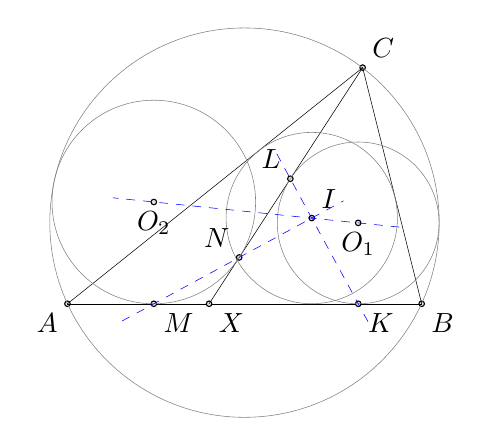
\begin{tikzpicture}[scale=1.5]
        \tkzDefPoints{0/0/A,3/0/B,2.5/2/C}
        \tkzDrawPoints(A,B,C) \tkzLabelPoints[below left](A) \tkzLabelPoints[below right](B) \tkzLabelPoints[above right](C)
        
        \tkzDefCircle[circum](A,B,C) \tkzGetPoint{O}
	\tkzDrawCircle(O,A)
	
	\tkzDrawSegments(A,C B,C A,B)
	\tkzDefPointWith[linear,K=0.4](A,B) \tkzGetPoint{X}
	\tkzDrawPoint(X) \tkzLabelPoints[below right](X)
	\tkzDrawSegment(C,X)
	
	\tkzDefTriangleCenter[in](A,B,C) \tkzGetPoint{I}
	\tkzDefCircle[in](A,B,C) \tkzGetPoints{I}{i}
	\tkzDrawPoints(I) \tkzLabelPoints[above right](I) \tkzDrawCircle(I,i)
	
	\tkzDefLine[bisector](C,X,B) \tkzGetPoint{x}
	
	\tkzDefLine[perpendicular=through I](X,x) \tkzGetPoint{c}
	
	\tkzInterLL(A,B)(I,c) \tkzGetPoint{K}
	\tkzInterLL(X,C)(I,c) \tkzGetPoint{L}
	
	\tkzDrawPoints(K,L) \tkzLabelPoints[below right](K) \tkzLabelPoints[above left](L)
	
	
	\tkzDefLine[perpendicular=through L](X,C) \tkzGetPoint{cc}
	\tkzDefLine[perpendicular=through K](A,B) \tkzGetPoint{ccc}
	
	\tkzInterLL(L,cc)(K,ccc) \tkzGetPoint{O_1}
	\tkzDrawCircle(O_1,K)
	\tkzDrawPoint(O_1) \tkzLabelPoints[below](O_1)
	
	\tkzDefLine[bisector](C,X,A) \tkzGetPoint{x'}
	
	\tkzDefLine[perpendicular=through I](X,x') \tkzGetPoint{c'}
	
	\tkzInterLL(A,B)(I,c') \tkzGetPoint{M}
	\tkzInterLL(X,C)(I,c') \tkzGetPoint{N}
	
	\tkzDrawPoints(M,N) \tkzLabelPoints[below right](M) \tkzLabelPoints[above left](N)
	
	\tkzDefLine[perpendicular=through N](X,C) \tkzGetPoint{cc}
	\tkzDefLine[perpendicular=through M](A,B) \tkzGetPoint{ccc}
	
	\tkzInterLL(N,cc)(M,ccc) \tkzGetPoint{O_2}
	\tkzDrawCircle(O_2,M)
	\tkzDrawPoint(O_2) \tkzLabelPoints[below](O_2)
	
	\tkzDrawLine[dashed, blue](O_1, O_2)
	
	\tkzDrawLines[dashed, blue](L,K M,I)
    \end{tikzpicture}
\end{center}

As it turns out this statement is true for arbitrary circles \(\omega_1\) and \(\omega_2\).

\begin{lemma}
	Let \(\omega_1\) and \(\omega_2\) be arbitrary circles prove that if \(LN\) is the inner tangent line between them and \(MK\) is the outer, then \(MN \cap LK \in O_1 O_2\).
\end{lemma}

This is a wonderful statement to consider on its own. Proving this statement automatically proves Thebault's theorem. Let us consider the homothepy center \(P\) which transforms \(\omega_1\) to \(\omega_2\) (in other words the intersection of the two outer common tangents). Let \(X\) and \(Y\) be the points of tangency of the common tangent of \(\omega_1\) and \(\omega_2\). Let \(A\) and \(B\) be the intersection of \(NL\) with \(MK\) and \(XY\) respectively. Consider the triangle \(\triangle ABP\), then \(\omega_1\) is its incircle and \(\omega_2\) is its excircle. Then, by the Iran lemma the projection of \(B\) onto the bisector of \(\angle{BPA}\) must lie on both \(MN\) and \(LK\).

\begin{center}
    \centering
    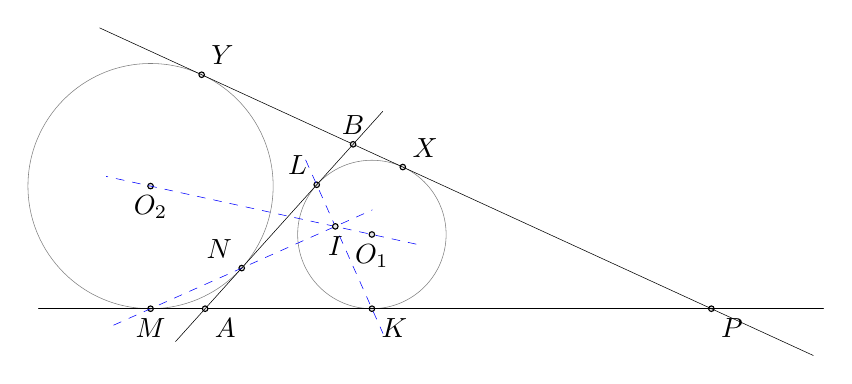
\begin{tikzpicture}[scale=1.5]
        \tkzDefPoints{0/0/A,3/0/B,3/2/C}
        
        \tkzDefCircle[circum](A,B,C) \tkzGetPoint{O}
		
	\tkzDefPointWith[linear,K=0.4](A,B) \tkzGetPoint{X}
	
	\tkzDefTriangleCenter[in](A,B,C) \tkzGetPoint{I}
	\tkzDefCircle[in](A,B,C) \tkzGetPoints{I}{i}
	
	\tkzDefLine[bisector](C,X,B) \tkzGetPoint{x}
	
	\tkzDefLine[perpendicular=through I](X,x) \tkzGetPoint{c}
	
	\tkzInterLL(A,B)(I,c) \tkzGetPoint{K}
	\tkzInterLL(X,C)(I,c) \tkzGetPoint{L}
	
	\tkzDrawPoints(K,L) \tkzLabelPoints[below right](K) \tkzLabelPoints[above left](L)
	
	
	\tkzDefLine[perpendicular=through L](X,C) \tkzGetPoint{cc}
	\tkzDefLine[perpendicular=through K](A,B) \tkzGetPoint{ccc}
	
	\tkzInterLL(L,cc)(K,ccc) \tkzGetPoint{O_1}
	\tkzDrawCircle(O_1,K)
	\tkzDrawPoint(O_1) \tkzLabelPoints[below](O_1)
	
	\tkzDefLine[bisector](C,X,A) \tkzGetPoint{x'}
	
	\tkzDefLine[perpendicular=through I](X,x') \tkzGetPoint{c'}
	
	\tkzInterLL(A,B)(I,c') \tkzGetPoint{M}
	\tkzInterLL(X,C)(I,c') \tkzGetPoint{N}
	
	\tkzDrawPoints(M,N) \tkzLabelPoints[below](M) \tkzLabelPoints[above left](N)
	
	\tkzDefLine[perpendicular=through N](X,C) \tkzGetPoint{cc}
	\tkzDefLine[perpendicular=through M](A,B) \tkzGetPoint{ccc}
	
	\tkzInterLL(N,cc)(M,ccc) \tkzGetPoint{O_2}
	\tkzDrawCircle(O_2,M)
	\tkzDrawPoint(O_2) \tkzLabelPoints[below](O_2)
	
	\tkzDrawLine[dashed, blue](O_1, O_2)
	
	\tkzDrawLines[dashed, blue](L,K M,I)
	
	\tkzDrawPoint(I) \tkzLabelPoints[below](I)
	
	\tkzInterLL(M,K)(O_1,O_2) \tkzGetPoint{P} 
	\tkzDrawPoint(P) \tkzLabelPoints[below right](P) \tkzDrawLine(M,P)
	
	\tkzDefLine[tangent from = P](O_1,K) \tkzGetPoints{XX}{X}
	\tkzDefLine[tangent from = P](O_2,M) \tkzGetPoints{YY}{Y}
	
	\tkzDrawPoints(X,Y) \tkzLabelPoints[above right](X,Y) \tkzDrawLine(P,Y)
	
	\tkzInterLL(L,N)(M,K) \tkzGetPoint{A} \tkzDrawPoint(A) \tkzLabelPoints[below right](A)
	\tkzInterLL(L,N)(X,Y) \tkzGetPoint{B} \tkzDrawPoint(B) \tkzLabelPoints[above](B)
	
	\tkzDrawLine(A,B)
    \end{tikzpicture}
\end{center}

In other words, the projection of \(B\) onto the bisector of \(\angle{APB}\) is \(MN \cap LK\). However, the projection of \(B\) onto the bisector of \(\angle{APB}\) obviously is part of \(O_1 O_2\). Thus, \(MN \cap LK \in O_1 O_2\) and the lemma is proven, proving Thebault's theorem.

\end{proof}

\end{document}
































